\documentclass{template/acm_proc_article-sp}

\usepackage{graphicx}
\usepackage[utf8]{inputenc}
\usepackage[english]{babel}
\usepackage{hyperref}
\usepackage{listings}
\usepackage{color}
\usepackage{siunitx}
\usepackage{csvsimple}
\usepackage{subcaption}
\usepackage{amsmath}

\begin{document} 

\title{Image tamper detection based on demosaicing artifacts}

\numberofauthors{2} 
\author{
% 1st. author 
\alignauthor
Matjaž Mav\\
       \affaddr{Faculty of Computer and Information Science, University of Ljubljana}\\
       \email{mm3058@student.uni-lj.si}
% 2nd. author
\alignauthor
Klemen Jesenovec\\
       \affaddr{Faculty of Computer and Information Science, University of Ljubljana}\\
       \email{kj9807@student.uni-lj.si}
}

\maketitle
\begin{abstract}
This paper reviews and summarizes research done on image tampering detection
using a color filter array demosaicing technique. The algorithm and it's features are
explained and implemented in MATLAB. The algorith is tested on sample data and results
are discussed.
\end{abstract}

\keywords{Image tampering, digital forensics, color filter array}

\section{Introduction}
This paper aims to review and summarize a paper about image tamper 
detection in the field of digital image forensics~\cite{dirik2009image}.

The paper classifies image tampering into three groups: 
\begin{description}
    \item[Targeted Tamper Detection] Which focus on detecting specific groups of 
    tampering such as re-compression, cloning, resizing, etc. 
    \item[Universal Tamper Detection] Which can only determine if the image
    was tampered with or not.
    \item[Localized Tamper Detection] Which can identify parts of the image 
    that were tampered with.
\end{description}

The paper describes a Color Filter Array (CFA) demosaicing based tamper detection
that can detect both local and universal tempering.
The method works due to the fact that image tampering usually alters CFA demosaicing
artifacts in a way that can be detected and can thus detect a wide range of tampering
techniques. 

In the following chapters we explain CFA, summarize the technique presented 
in the original paper and present our own implementation in MATLAB.
Finally, we discuss the results and limitations of our implementation and compare it
to the results in the original paper.

\section{Color filter array}
Color filter array is a grid of small color 
filters put over an image sensor~\cite{cfawiki}.
The filters are needed due to the sensor's inability to capture wavelength 
information and thus cannot distinguish between different colors.
The CFA filters out specific colors before the light arrives at the image sensor.
This enables cameras to capture color information.

There are many types of CFA although the Bayer filter is most commonly used and is 
illustrated in figure~\ref{img_4_bayer_filters}.
It uses one red, one blue and 2 green filters per pixel. 
Green being used twice due to human eye sensitivity to green color.

Other types of filters include a RGBE filter which also uses an emerald filter, a CYYM
filter which uses one cyan, two yellow and one magenta filter, a RGBW filter which also uses a white filter, etc.

The process of interpolating different sets of color information into a single image 
is called demosaicing~\cite{demowiki}.

\begin{figure}
\centering
\includegraphics[trim=175 200 100 205,clip,width=0.46\textwidth]{report/results/4_bayer_filters.jpg}
\caption{Commonly used Bayer filters}
\label{img_4_bayer_filters}
\end{figure}

\section{CFA Interpolation}
CFA interpolation or demosaicing is the process of building a singe image from
multiple color sets~\cite{demowiki}. 
This can be achieved using simple interpolation techniques such as 
nearest-neighbor interpolation~\cite{nnwiki}, bilinear interpolation~\cite{bilwiki}, 
bicubic interpolation~\cite{bicwiki}, spline interpolation~\cite{splinewiki}, etc.

Advanced demosaicing algorithms using pixel correlation such as 
variable number of gradients, pixel grouping, adaptive homogeneity-directed
are out of scope of this paper.

Bilinear interpolation is used in this paper as it was also used in
the original paper. The original paper also states result do not
differ using bicubic interpolation.


\section{CFA based features}
In this section we will review two CFA based features introduced in the paper \cite{dirik2009image}. The first feature (referred to as  $F_1$) mainly relies on the estimation of the source digital camera CFA pattern. And the second feature (referred to as $F_2$) relies on the source digital camera sensor noise.

Both of the features can be used in universal tampering detection and also when applied with sliding window in local tampering detection.

For both of the features we implemented algorithm in MATLAB. All code is available on the GitHub repository\\\textit{matjazmav/fri-1819-df-seminar}\footnote{\url{https://github.com/matjazmav/fri-1819-df-seminar}}.

\subsection{Feature 1: Pattern number estimation}
This feature is trying to estimate which CFA pattern was used by the source digital camera.

To estimate possible used CFA pattern, the image is first re-sampled with each of the CFA patterns (usually only 4 most commonly used that are illustrated in figure \ref{img_4_bayer_filters}) and then re-interpolated with the same CFA pattern. This steps are illustrated in figure \ref{img_f1_steps}. After that (3) MSE between the image and its re-interpolated part is calculated. For the image that is not tampered, one of the MSE values are expected to be significantly smaller from the others. If that is not the case, the image may have been post-processed.

We followed steps that are introduced in referenced paper \cite{dirik2009image} and implemented MATLAB algorithm that estimates $F_1$ feature. Unfortunately we ware not able to reproduced the results that are described in there.

\begin{figure}
\centering

\begin{subfigure}{0.23\textwidth}
    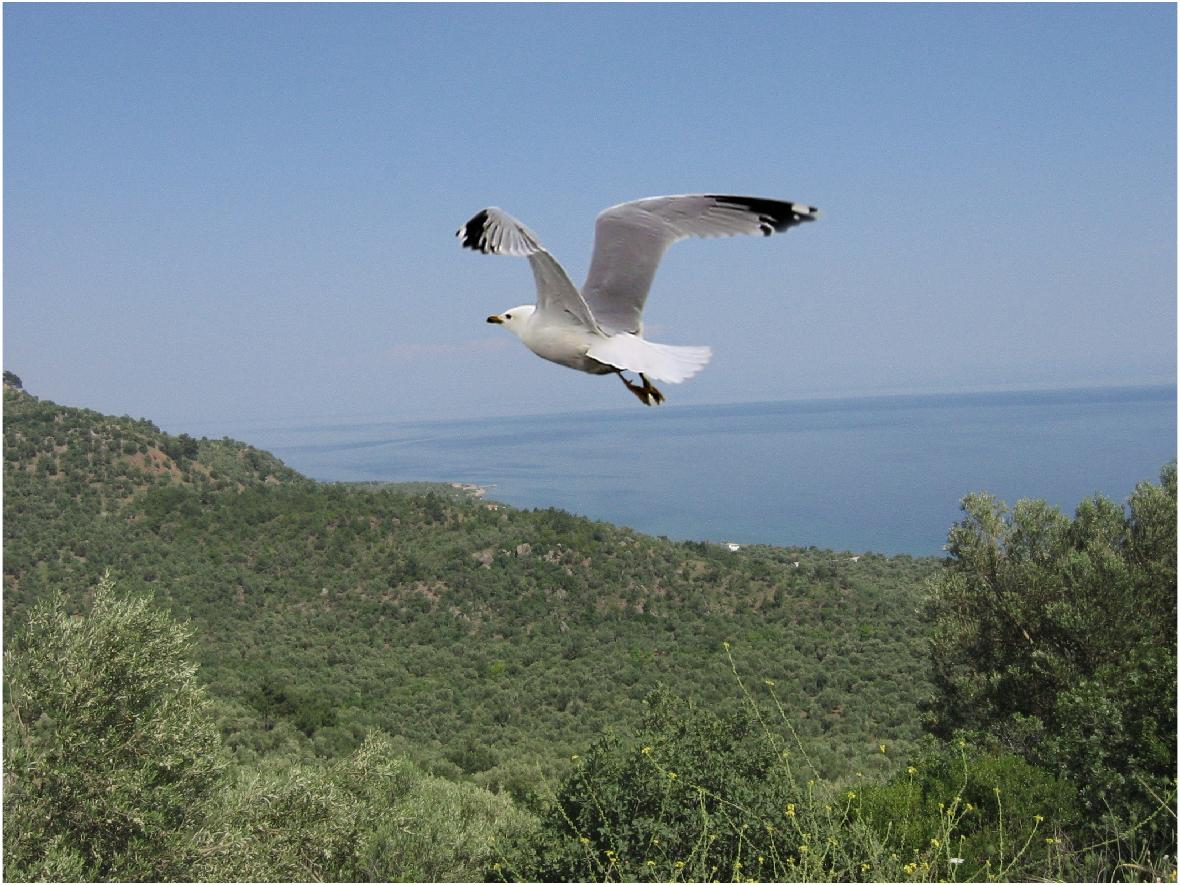
\includegraphics[trim=0 0 0 0,clip,width=\linewidth]{report/results/f1_steps_0.jpg}
    \caption{Original image}
\end{subfigure}
\hspace*{\fill}
\begin{subfigure}{0.23\textwidth}
    
\includegraphics[trim=0 0 0 0,clip,width=\linewidth]{report/results/f1_steps_1.jpg}
    \caption{CFA filter}
\end{subfigure}

\begin{subfigure}{0.23\textwidth}
    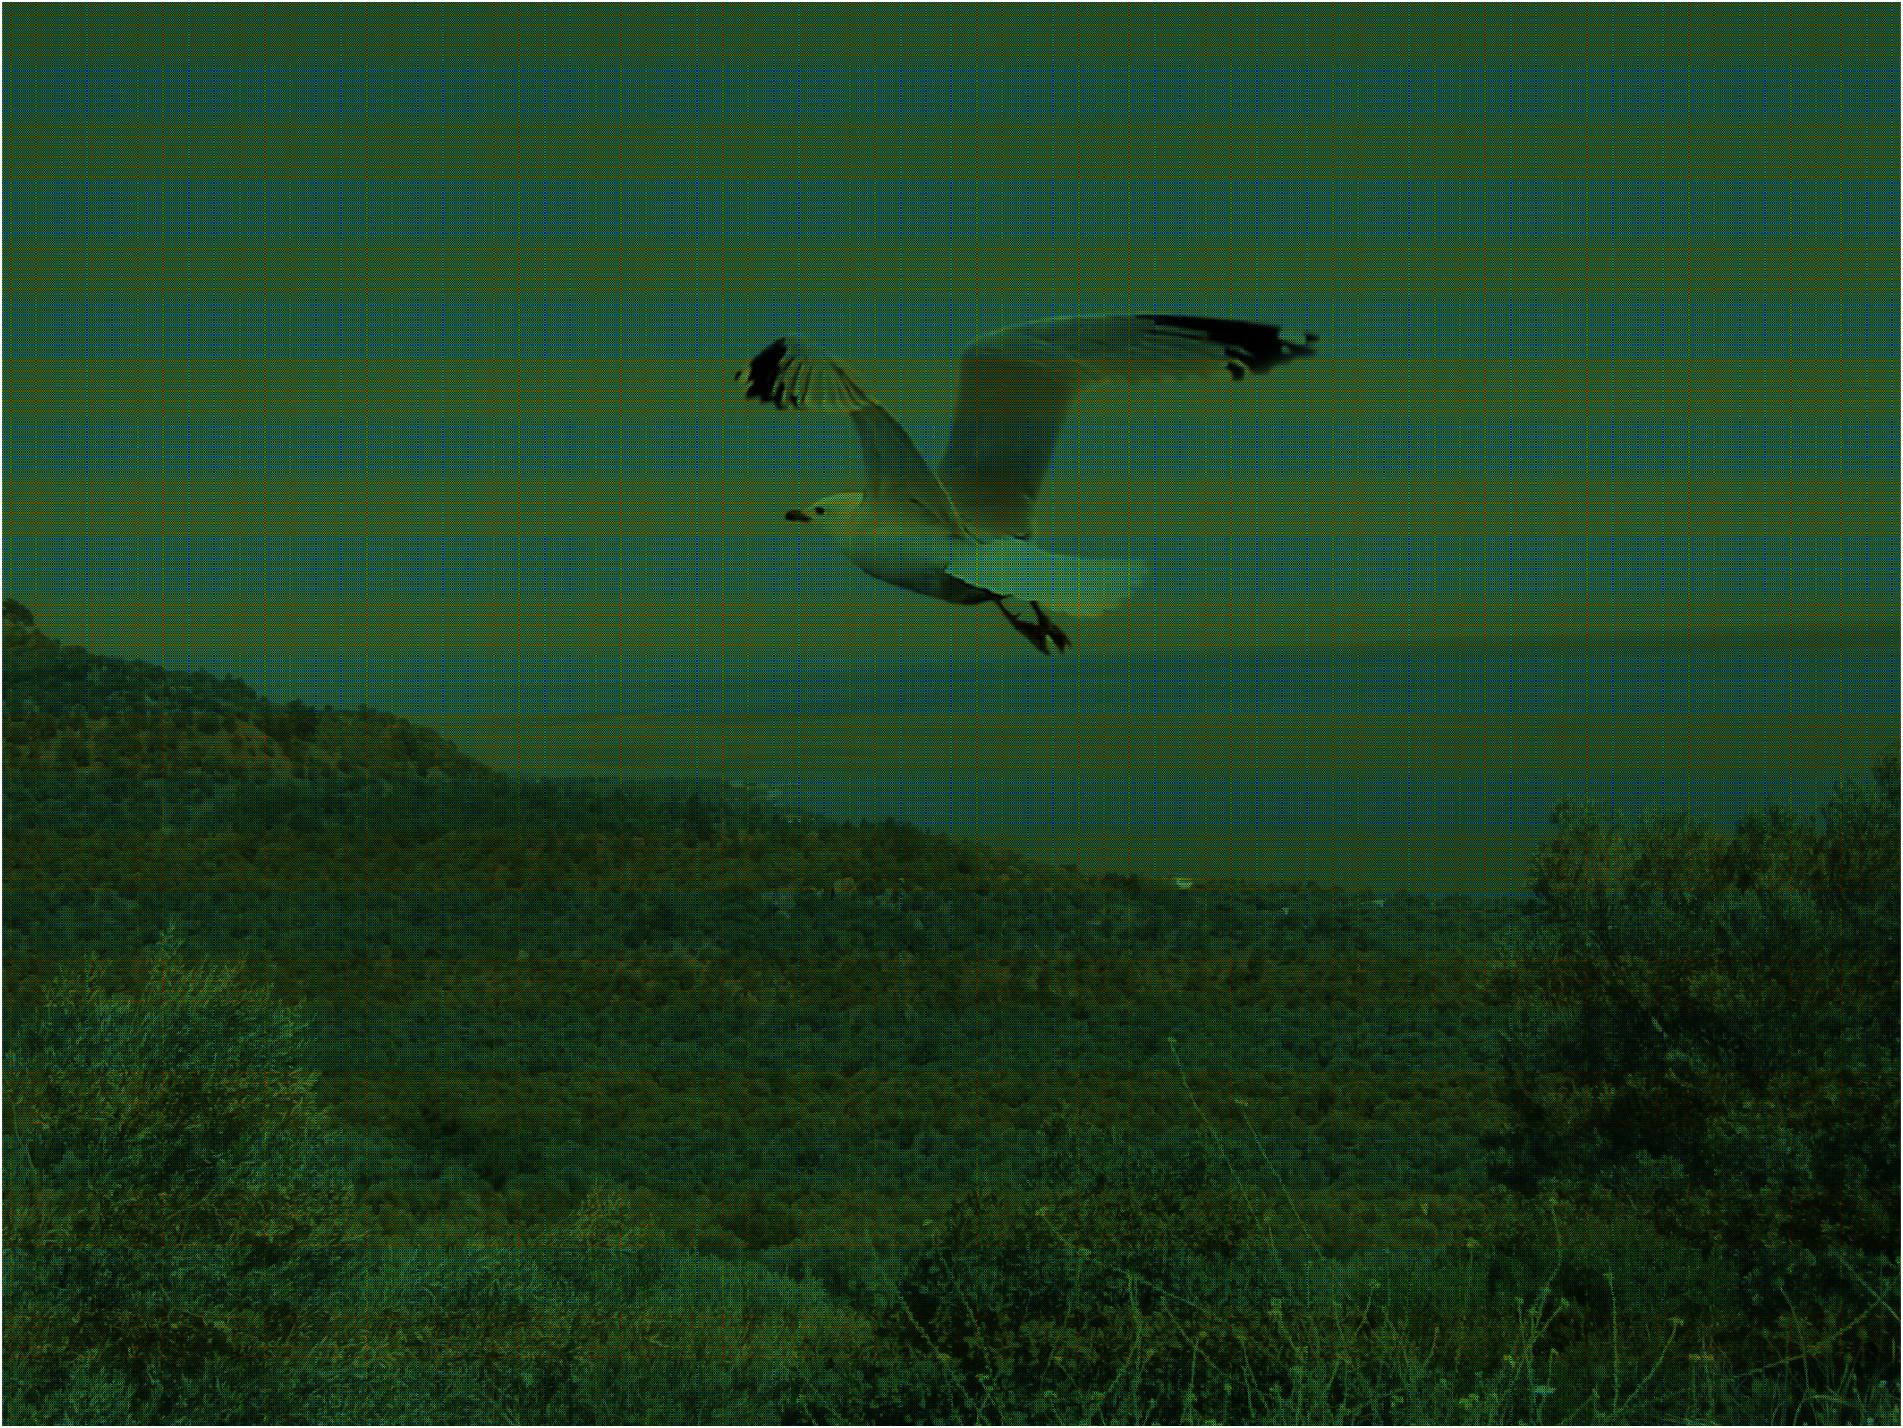
\includegraphics[trim=0 0 0 0,clip,width=\linewidth]{report/results/f1_steps_2.jpg}
    \caption{Re-sampled image}
\end{subfigure}
\hspace*{\fill}
\begin{subfigure}{0.23\textwidth}
    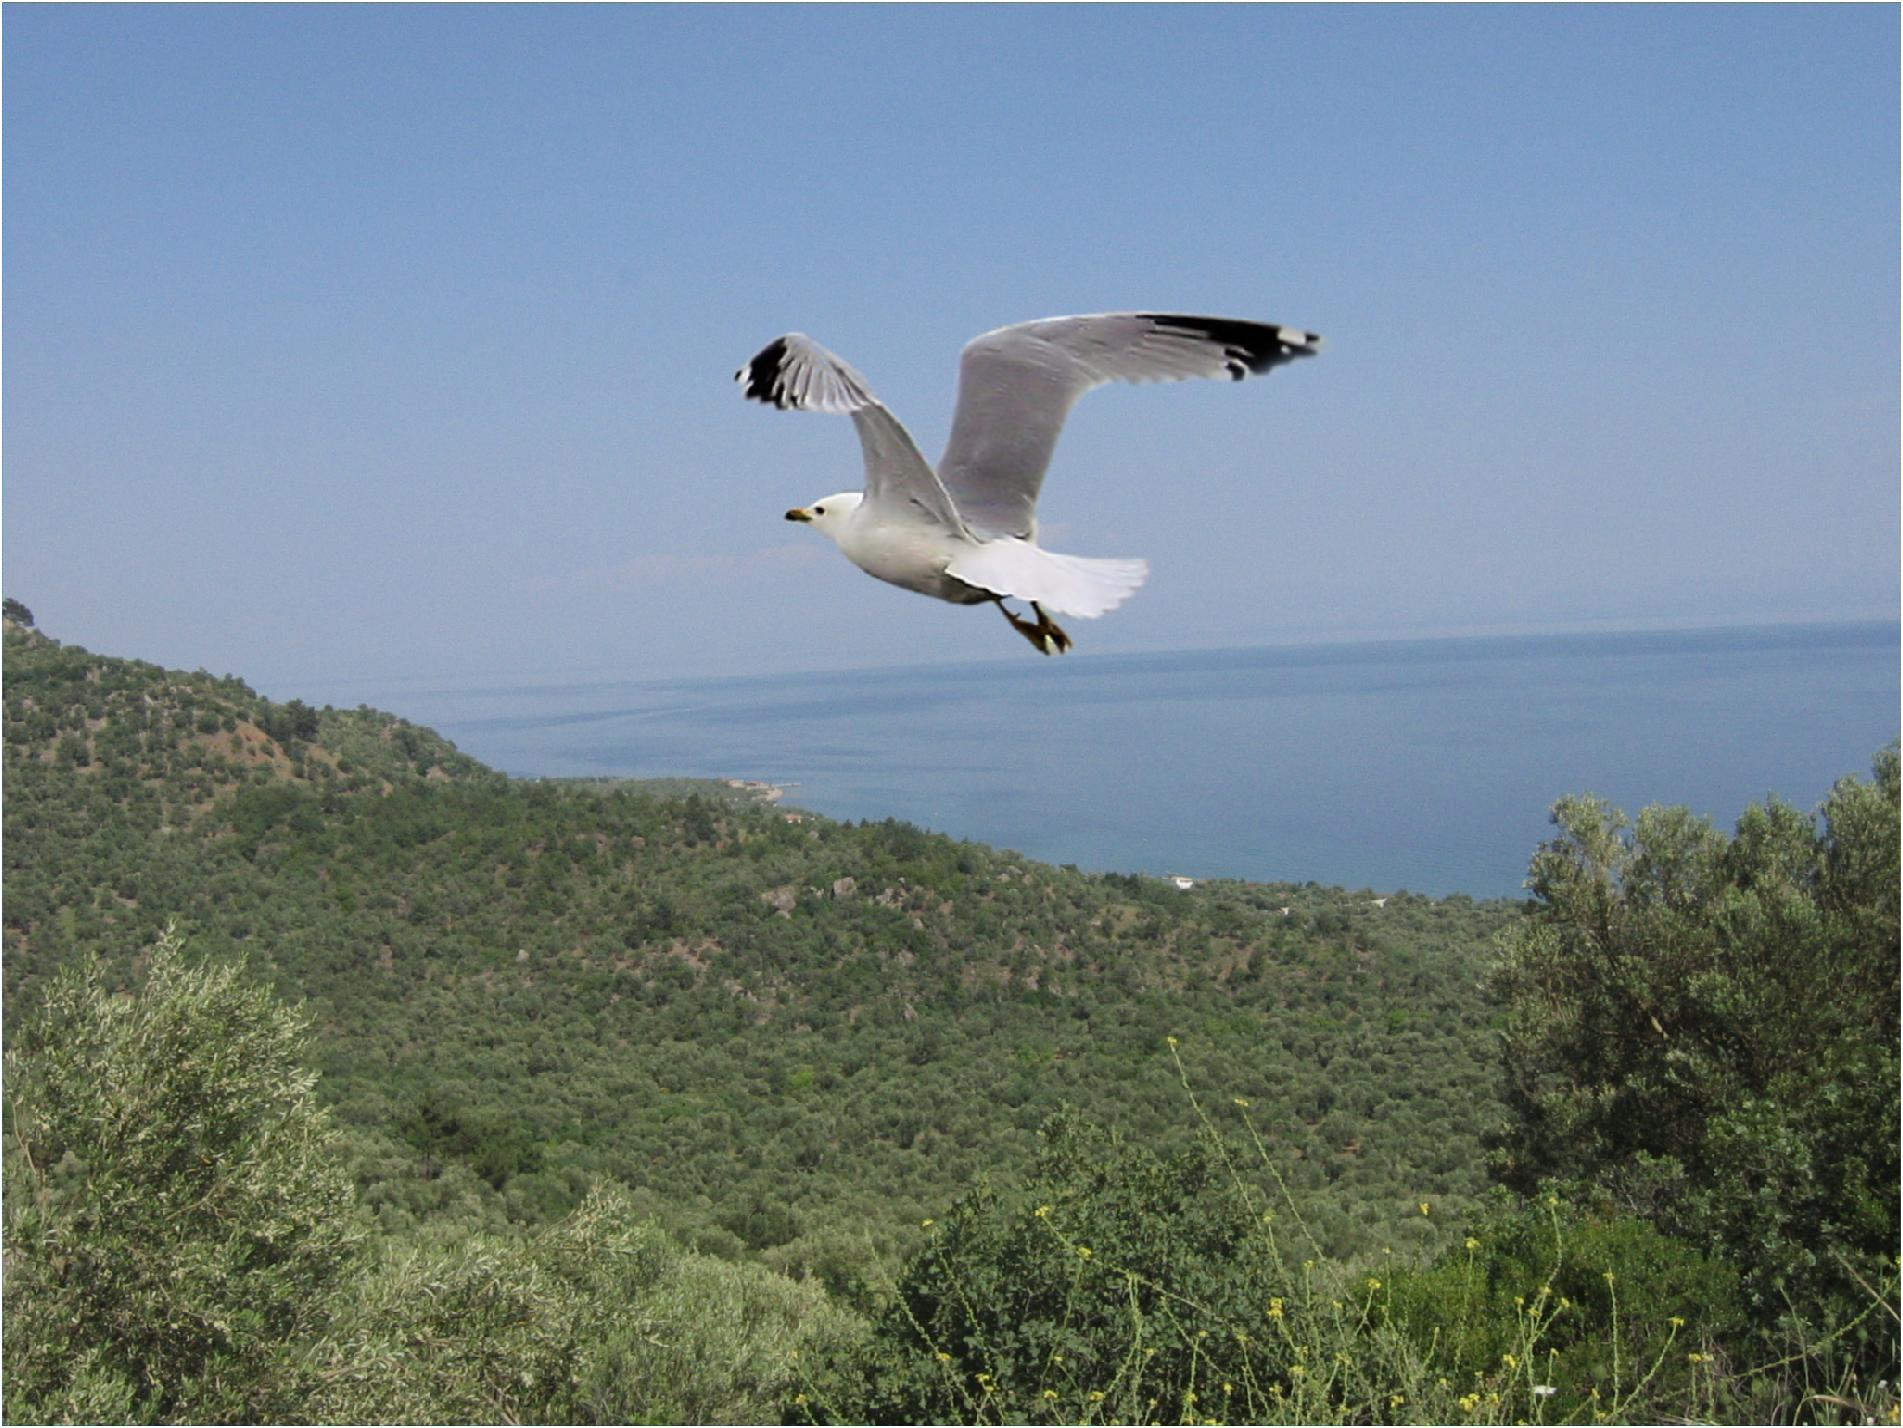
\includegraphics[trim=0 0 0 0,clip,width=\linewidth]{report/results/f1_steps_3.jpg}
    \caption{Re-interpolated image}
\end{subfigure}

\caption{Steps taken in $F_1$ feature estimation. Original image (a) and selected CFA filter (b) are used to re-sample image. The re-sampled image (c) is then re-interpolated with the selected CFA filter (b). Final result is shown in (d).}
\label{img_f1_steps}
\end{figure}

\subsection{Feature 2: CFA based noise analysis}
\label{sec_f2}
This feature analyses the source digital camera noise. If the image is CFA interpolated the variance of the CFA interpolated pixels is expected to be significantly smaller that the variance of non-interpolated pixels.

To calculate $F_2$ feature we need to follow this steps:
\begin{enumerate}
    \item Estimate sensor noise on the green channel of the image. First denoise image with level 1 wavelet denoising. Noise is defined as difference between image and corresponding denoised image.
    \item Calculate variance of the estimated noise of the interpolated $A_1$ and corresponding non-interpolated $A_2$ pixels.
    \item The final $F_2$ feature is calculated as maximum between both variance ratios (equation \ref{eq_f2}).
\end{enumerate}

\begin{align}
F_2 = max(\frac{var(A_1)}{var(A_2)}, \frac{var(A_2)}{var(A_1)})
\label{eq_f2}
\end{align}

Our MATLAB implementation of the $F_2$ feature extraction for the global tampering detection follows as:

\begin{lstlisting}[language=Matlab,basicstyle=\tiny,numberstyle=\tiny,numbers=left,numbersep=5pt]
function f2 = extract_f2(I)
% INPUTS
% I - RGB image
% OUTPUTS
% f2 - f2 measure

[h,w,~] = size(I);

G = double(I(:,:,2)); % extracted green color channel
Gd = wdenoise2(G,1);  % denoise image
N = G - Gd;           % extract image noise            

% resize green color mask
mask = logical(repmat([1 0; 0 1], ceil([h/2 w/2])));
mask = mask(1:h, 1:w);

A1 = N .* mask;       % extract non-interpolated noise vector
A2 = N .* ~mask;      % extract interpolated noise vector

% calculate f2 measure
vA1 = var(A1(:));
vA2 = var(A2(:)); 
f2 = max(vA1/vA2, vA2/vA1);

end;
\end{lstlisting}

With slight modification of upper implementation, lines 13 - 23 ware processed with sliding window (using function \verb blockproc), we ware able to calculate $F_2$ map and successfully localize tampering on the two images that ware used in referenced paper.

\section{Experiments}
We evaluated both of the features on dataset used in referenced paper \cite{dirik2009image}, copy-move dataset MICC-F220 dataset \cite{amerini2011sift} that contains 110 pristine and 110 tampered images and also on small dataset that we prepared\footnote{Available on the GitHub repository in folder \textit{resources/datasets/ours}.}.

\subsection{Local tampering detection}

As we described in section \ref{sec_f2}, we ware able to successfully replicate the local tampering detection on the images used in the referenced paper \cite{dirik2009image}. The results of the our implementation are illustrated on the figure \ref{img_f2_localization}. Since our results are very similar to the results illustrated in the referenced paper we assume that our implementation is correct. 

Unfortunately we ware unable to successfully localize tampered regions on other datasets. 
\begin{figure}
\centering

\begin{subfigure}{0.46\textwidth}
    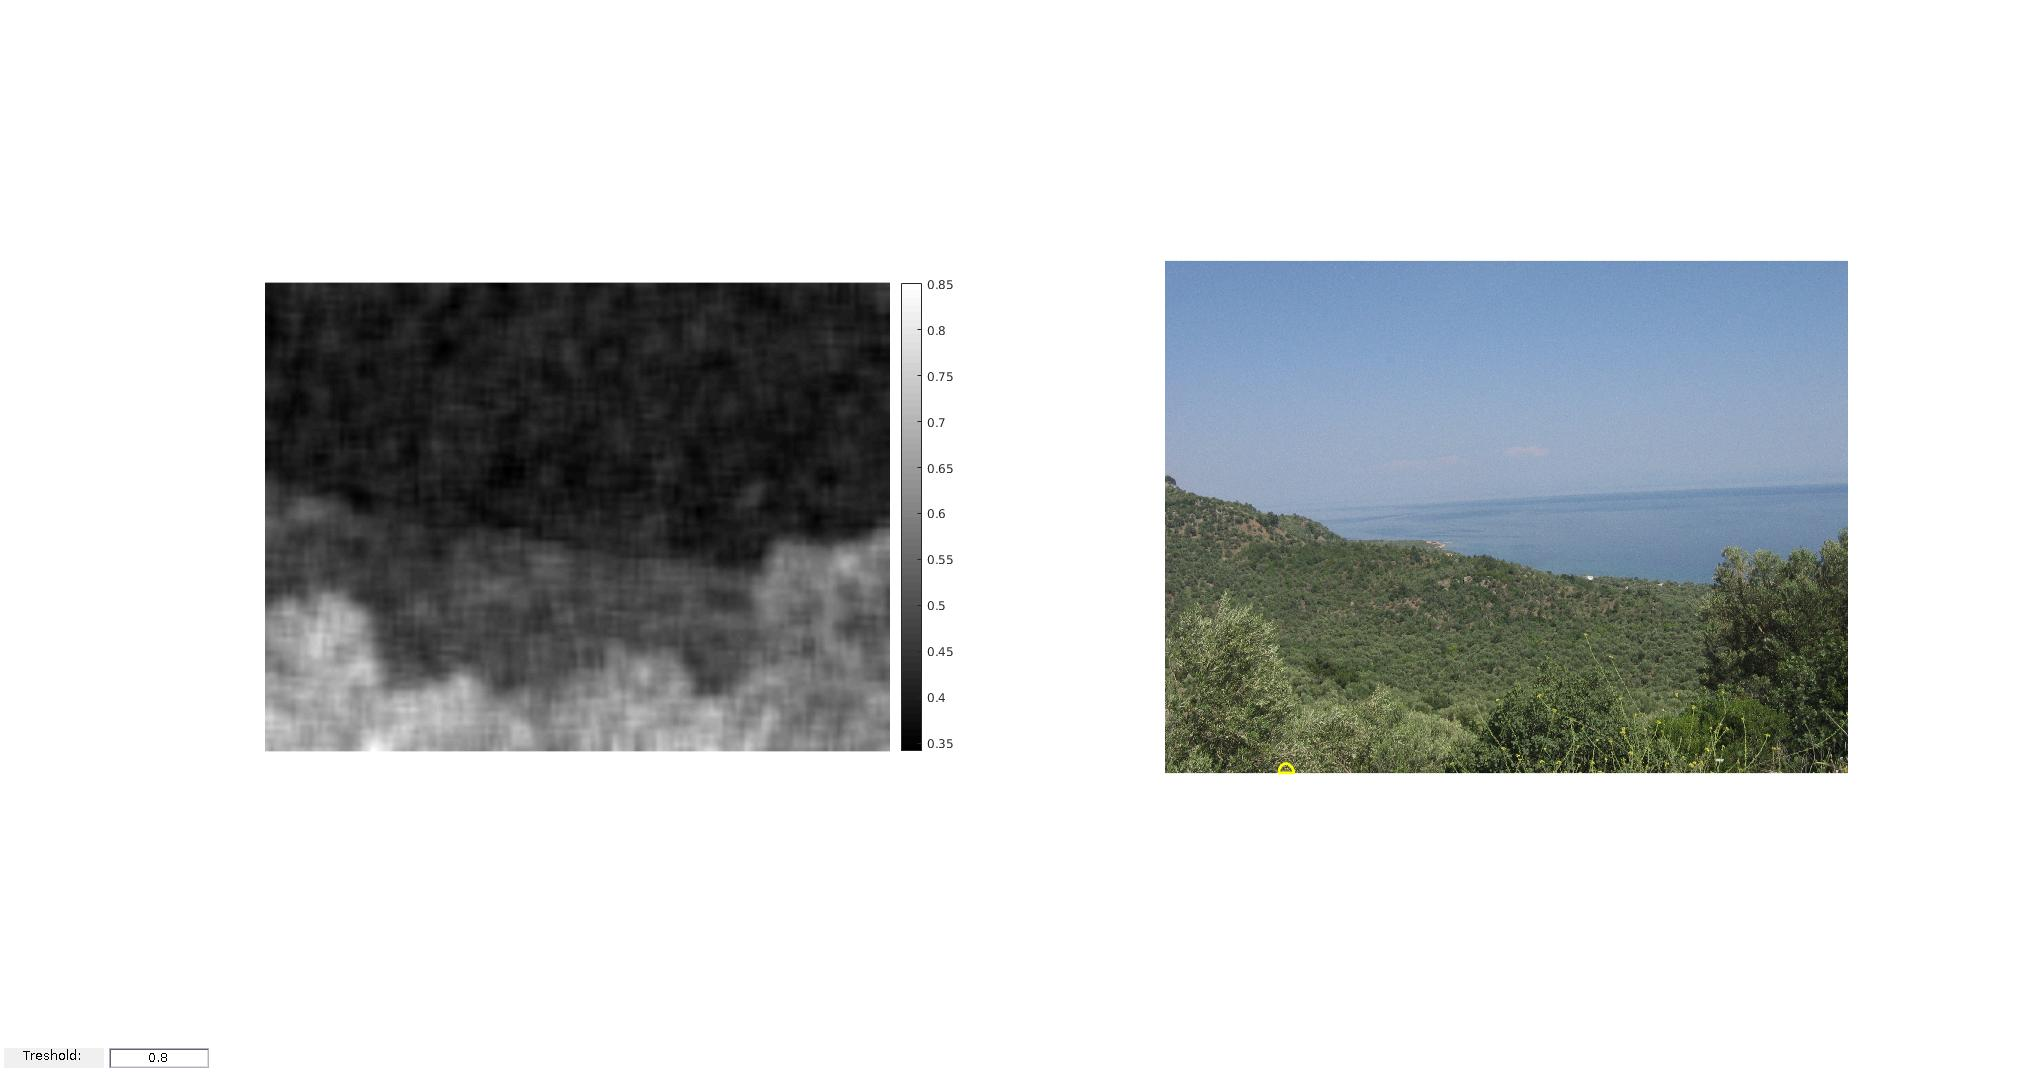
\includegraphics[trim=275 300 200 250,clip,width=\linewidth]{report/results/f2_seagull_orig.jpg}
    \caption{Pristine coast image}
\end{subfigure}

\begin{subfigure}{0.46\textwidth}
    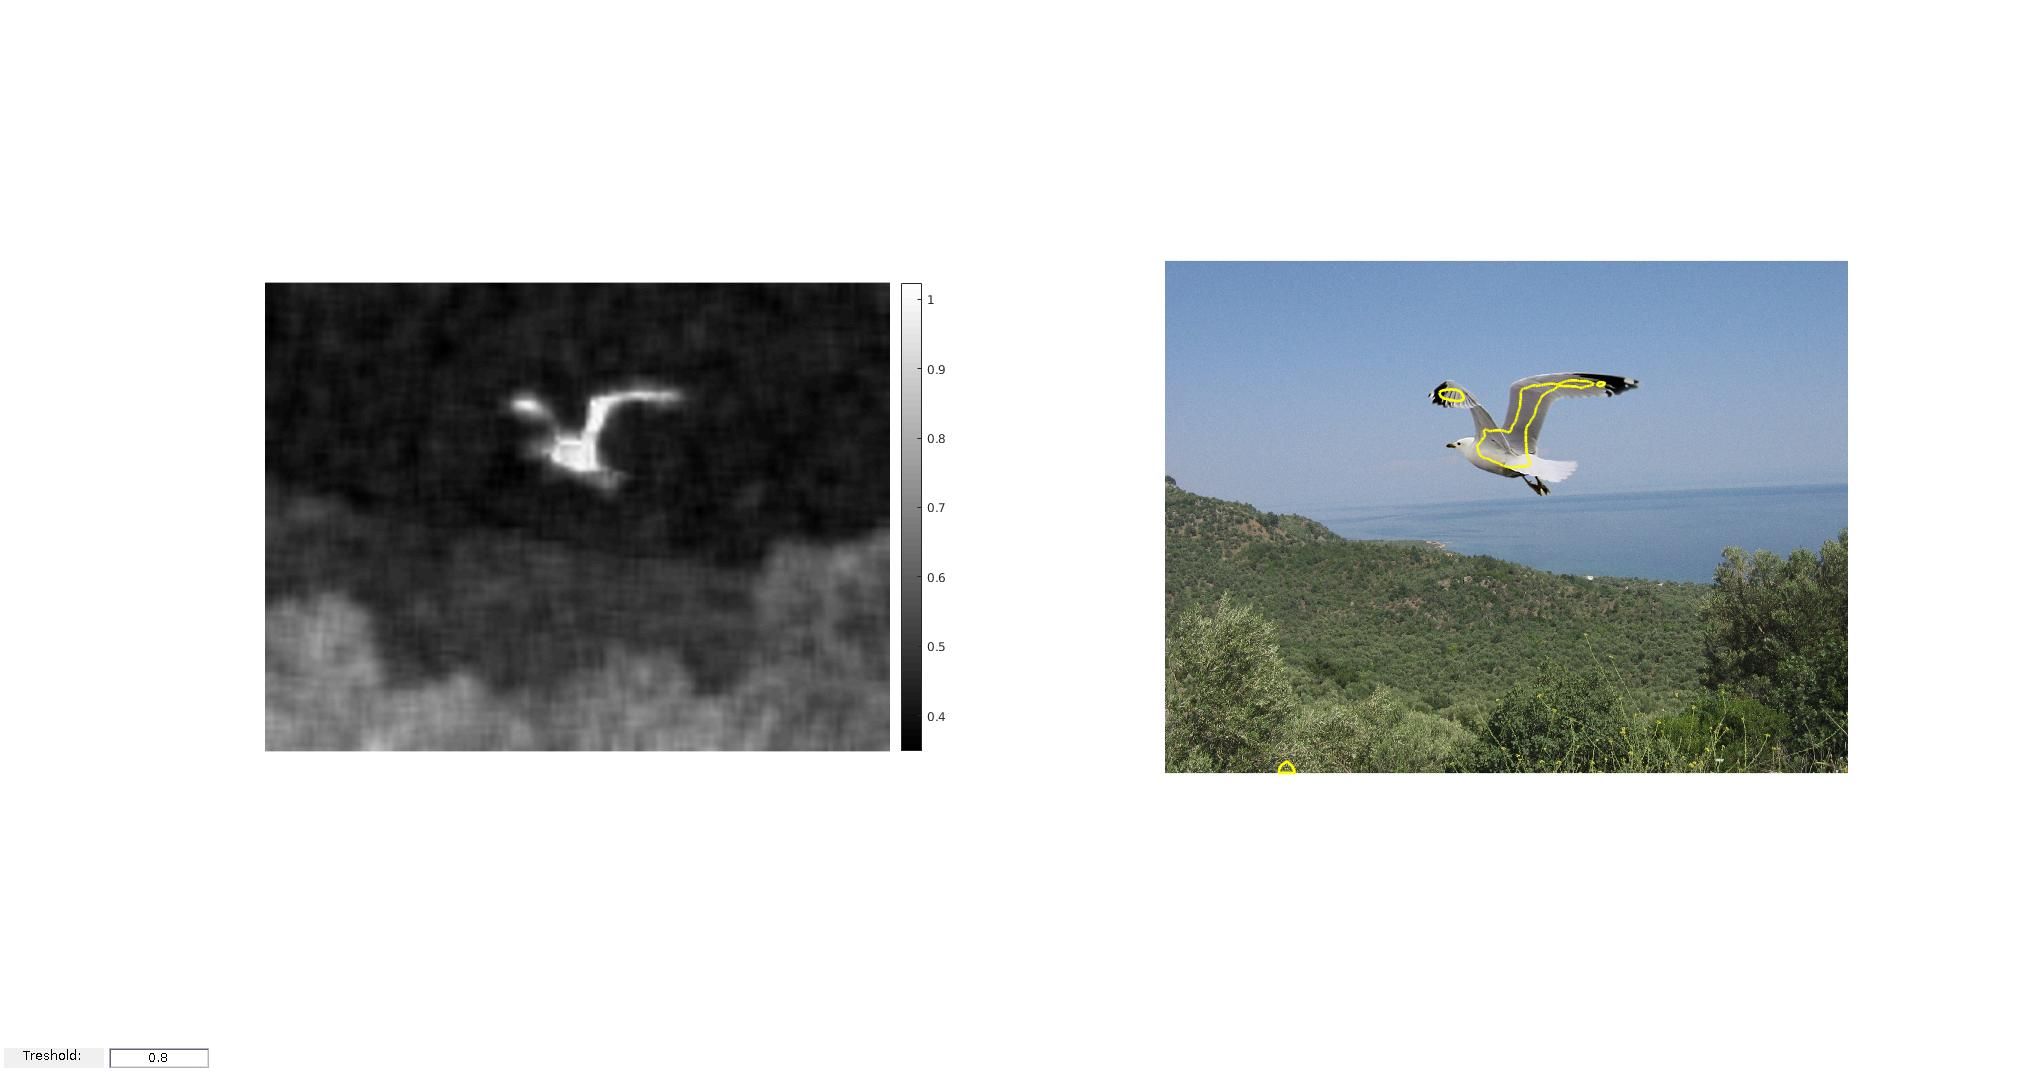
\includegraphics[trim=275 300 200 250,clip,width=\linewidth]{report/results/f2_seagull.jpg}
    \caption{Tampered coast image}
\end{subfigure}

\begin{subfigure}{0.46\textwidth}
    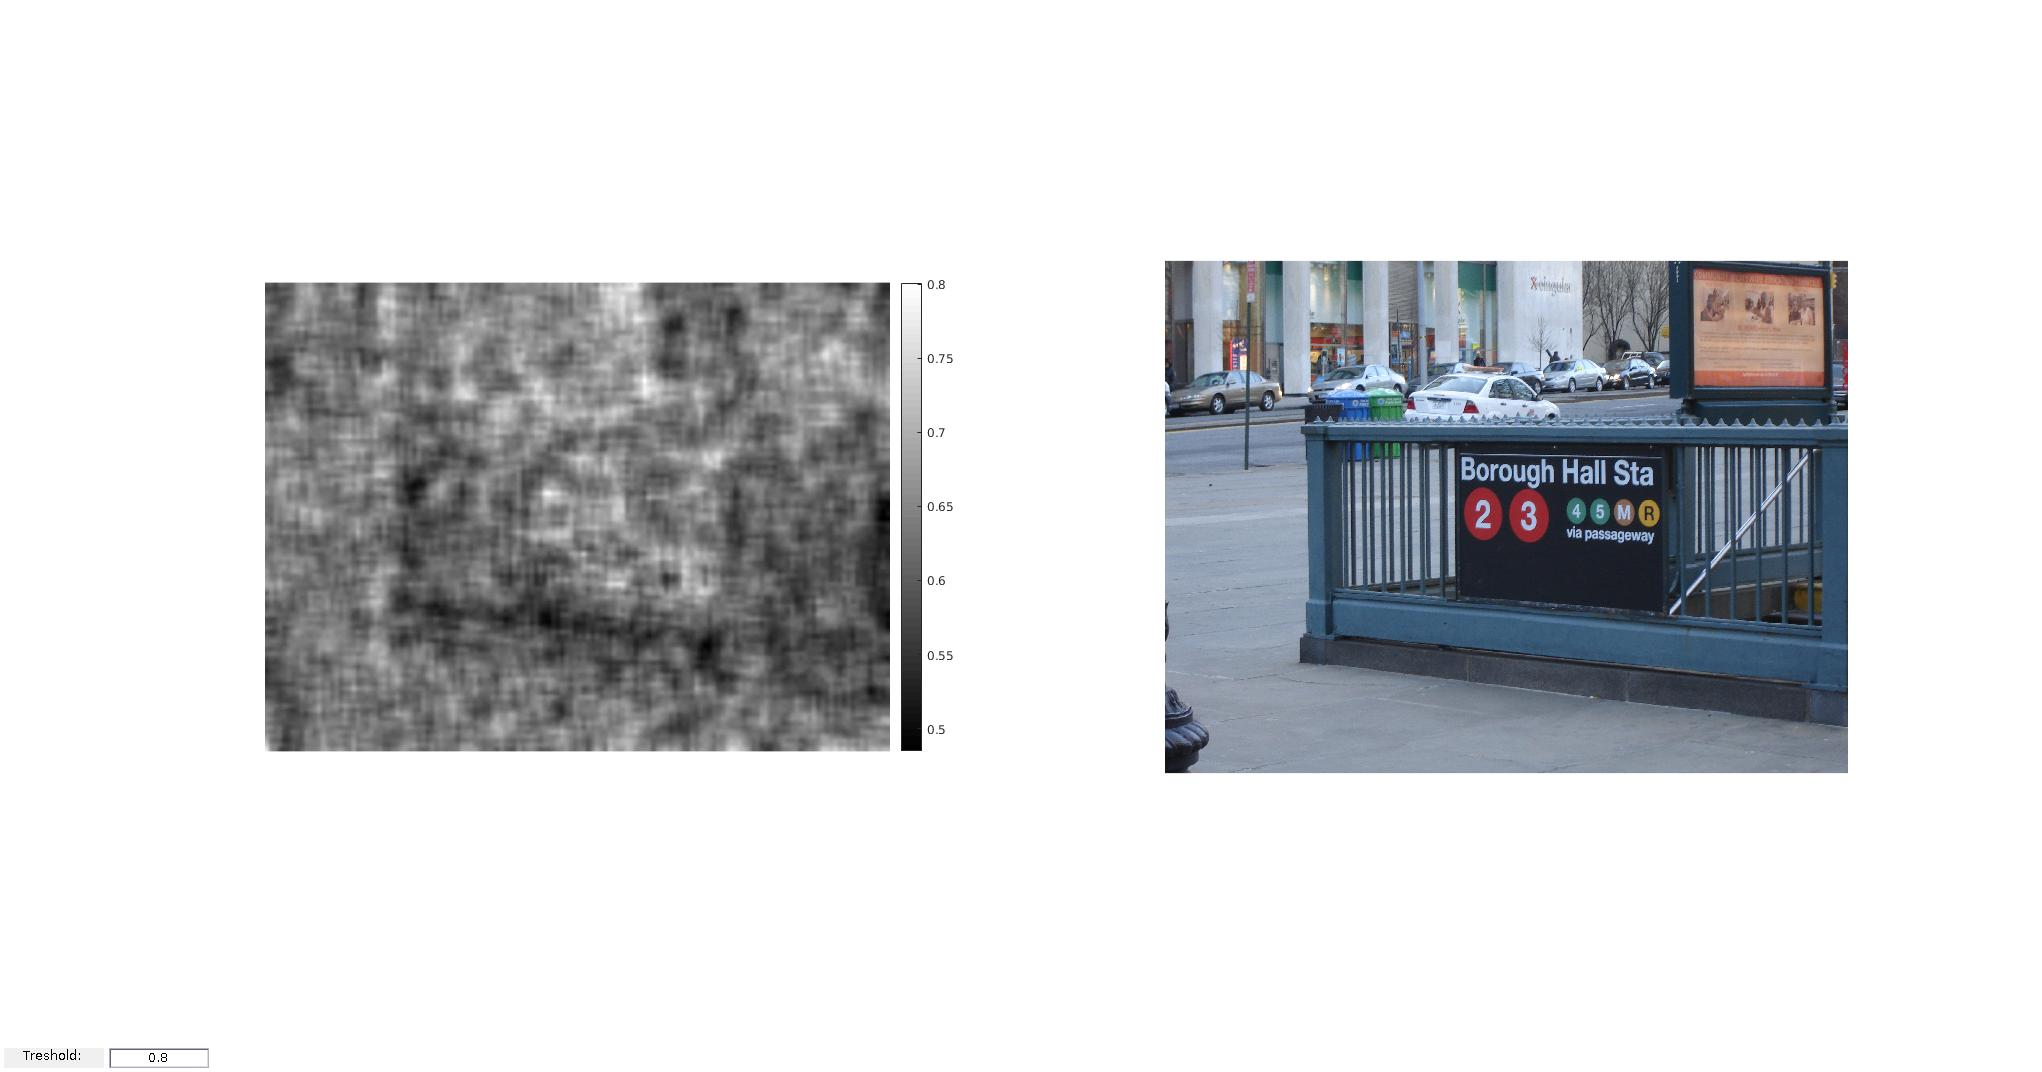
\includegraphics[trim=275 300 200 250,clip,width=\linewidth]{report/results/f2_subway_orig.jpg}
    \caption{Pristine subway entrance image}
\end{subfigure}

\begin{subfigure}{0.46\textwidth}
    \includegraphics[trim=275 300 200 250,clip,width=\linewidth]{report/results/f2_subway.jpg}
    \caption{Tampered subway entrance image}
\end{subfigure}

\caption{Local tampering detection with $F_2$ feature. Left images visualize $1/F_2$ map and right images are annotated where map is greater then threshold $T = 0.8$.}
\label{img_f2_localization}
\end{figure}

\subsection{Universal tampering detection}

TODO: we failed here + plot results on dataset

\section{Conclusions}
As seen in the results we were able to reproduce the results achieved in the 
original paper. However we were not able to detect tampering on other datasets.
This could be a result of ...
We were however successful in presenting and summarizing the techniques used.

\bibliographystyle{abbrv}
\bibliography{main}

\end{document}
